\documentclass[14pt,a4paper]{extreport}
\usepackage[utf8]{vietnam}
\usepackage{graphicx}
\usepackage{xcolor}
\usepackage{wrapfig}
\usepackage{multicol}
\usepackage{fancyhdr}
\usepackage{fancybox}
\usepackage{iflang}
\usepackage{caption}
\usepackage{amsmath}
\DeclareMathOperator*{\argmax}{argmax}
\DeclareMathOperator*{\argmin}{argmin}
\usepackage[left=2.5cm, right=2.50cm, top=2.50cm, bottom=2.50cm]{geometry}
\pagestyle{fancy}
\fancyhf{}
\fancyhead[LE,RO]{\thepage}
\fancyhead[LO]{\small{\itshape{}}}
\graphicspath{ {./images/} }
\begin{document}


	\thispagestyle{empty}
\thisfancypage{
	\setlength{\fboxsep}{10pt}
	\fbox}{}
\begin{center}
	\begin{large}
		TRƯỜNG ĐAI HỌC BÁCH KHOA HÀ NỘI
	\end{large} \\
	\begin{large}
		VIỆN CÔNG NGHỆ THÔNG TIN VÀ TRUYỀN THÔNG
	\end{large} \\
	
	\textbf{--------------------  *  ---------------------}\\[1.5cm]
	
\includegraphics[scale=0.25]{12}
	\\
	\vspace{1.5cm}
	{\fontsize{17pt}{1}\selectfont  Môn học}\\[0.3cm]
	{\fontsize{20pt}{1}\selectfont 	Lí thuyết ngôn ngữ và phương pháp dịch}\\[0.9cm]
	{\fontsize{17pt}{1}\selectfont  Tên đề tài}\\[0.5cm]
	{\fontsize{23pt}{1}\selectfont \textbf{Tìm hiểu về FLEX}}\\[1.3cm]
\end{center}
\vspace{1.5cm}
%\hspace{2.7cm}
\begin{center}
	{\fontsize{17pt}{1}
	\selectfont Giảng viên hướng dẫn: } \hspace{1pt}
\textbf{\parbox[t]{6cm}{
		\selectfont TS. Phạm Đăng Hải\\
	}
}
\end{center}

\hspace{1.59cm}
{\fontsize{17pt}{1}
	\selectfont Sinh viên thực hiện: } \hspace{1pt}
\textbf{\parbox[t]{6cm}{
		\selectfont Phạm\ Minh\ Tâm\\
		\selectfont Lâm\ Xuân\ Thư\\		
	}
}

\hspace{5.0cm}
%{\fontsize{12pt}{1}
%		\selectfont MSSV : } \hspace{1pt}
%	\textbf{\parbox[t]{6cm}{
%			\selectfont  20153709\\
%		}
%	}

\hspace{5.4cm}
{\fontsize{17pt}{1}
	\selectfont Lớp: } \hspace{1pt}
\textbf{\parbox[t]{6cm}{
		\selectfont KSTN\ CNTT\ K60\\
	}
}\\[20pt]

\vspace{1cm}
\begin{center}
	
	{\fontsize{17pt}{1}\selectfont Hà Nội, \today}
	%{\fontsize{12pt}{1}\selectfont November, 29$^{th}$, 2017}
\end{center}




\newpage
\thispagestyle{empty}
\tableofcontents 
%\listoffigures
\newpage
\setlength{\parindent}{4em}
\setlength{\parskip}{1em}
\renewcommand{\baselinestretch}{1.5}

%\begin{abstract}
%	content...
%\end{abstract}

\chapter{Giới thiệu flex}
\section{Tổng quan về flex}
$ flex $ là một công cụ dùng để sinh các $ scanner $. Một $ scanner $ là một chương trình nhận dạng các mẫu từ vựng (lexical patterns) trong một văn bản. Chương trình $ flex $ đọc các file đầu vào được cho trước, hoặc đầu vào mặc định nếu không có tên file nào được cung cấp, như là mô tả của một scanner sẽ được sinh. Mô tả này có dạng các cặp biểu thức chính quy và code C, gọi là các luật. $ flex $ sinh ra một file C ở output, mặc định là $ lex.yy.c $, dùng để định nghĩa hàm $ yylex() $. File này có thể được compile và link với flex runtime library để tạo ra một file thực thi. Khi ta chạy file thực thi, nó phân tích đầu vào dựa trên sự xuất hiện của các biểu thức chính quy. Bất cứ khi nào nó tìm thấy một biểu thức chính quy thoả mãn, nó sẽ thực thi phần code C tương ứng với biểu thức đó. 

Dưới đây là một ví dụ đầu vào của flex. Scanner được sinh ra ở ví dụ này có chức năng đếm số lượng kí tự và số lượng dòng trong input của nó. Output của nó đơn giản chỉ in ra số lượng kí tự và dòng đếm được. Dòng đầu tiên khai báo hai biến toàn cục và chúng có thể truy cập được trong cả hàm yylex() và main() được khai báo ở sau '\%\%" thứ hai. Có hai luật, một luật nhận dạng kí tự xuống dòng ('$ \setminus$n') và tăng cả số dòng cà số kí tự, và một luật nhận dạng kí tự bất kì khác kí tự xuống dòng (biểu thức '.').\\

\textit{ int num\_lines = 0, num\_chars = 0;\\
    \%\% \\
$ \setminus$n  \hspace{1cm}     ++num\_lines; ++num\_chars;\\
.  \hspace{1.4cm}     ++num\_chars; \\
\%\% \\
int main() \\
\{\\
	yylex();\\
	printf( "\# of lines = \%d, \# of chars = \%d", num\_lines, num\_chars );\\
\}}\\




\section{Sử dụng flex xây dựng bộ phân tích cho ngôn ngữ PL/0}

\begin{figure}
	\centering
	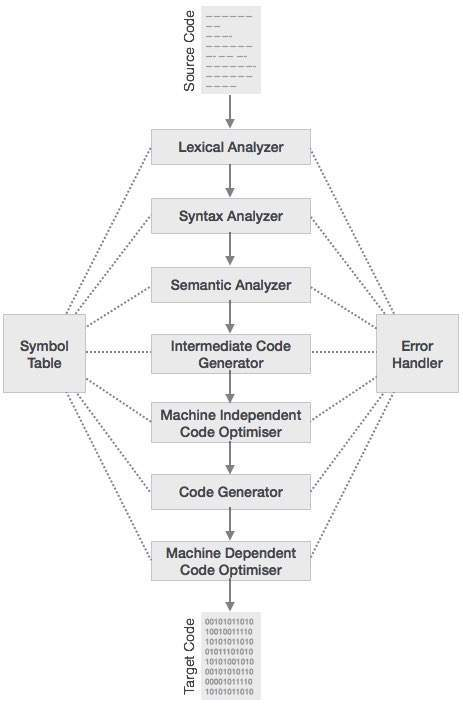
\includegraphics[scale=.6]{compiler_phases}
	\caption{Compiler phases}
\end{figure}

Quá trình biên dịch một chương trình là một chuỗi tuần tự các pha. Mỗi pha lấy đầu vào từ pha trước, và đưa ra output cho pha tiếp theo trong compiler. 

Trong đó pha đầu tiên (Lexical Analyzer) hoạt động như một text scanner. Pha này scan suorce code như một dòng liên tiếp các kí tự. Nó duyệt từng ký tự của văn bản nguồn, loại bỏ các ký tự không cần thiết như dấu cách, chú thích,.. Sau đó xây dựng từ vựng từ những ký tự đọc được, nhận dạng từ tố và gửi tới pha tiếp. 
 
Trong bài này chúng em sẽ trình bày các đặc trưng của flex và sau đó sử dụng flex để tạo ra một scanner thực hiện chức năng phân tích từ vựng cho ngôn ngữ PL/0.

\chapter{Cấu trúc file đầu vào flex}
File đầu vào flex có ba phần defintions, rules và user code, ngăn cách với nhau bởi một dòng chứa duy nhất '\%\%'.\\
\textit{defintions\\
\%\% \\
rules\\
\%\% \\
user code}

Cụ thể mỗi phần như sau:

\section{Defintions}
Phần definition chứa các khai báo định nghĩa tên, khai báo các điều kiện bắt đầu.

Định nghĩa tên có dạng: $ name $ $ definition $.\\
Trong đó, 'name' là một từ bắt đầu bởi một chữ cái hoặc một dấu gạch dưới ('\_'), sau đó là không có hoặc nhiều chữ cái, chữ số, gạch dưới hoặc dấu '-' (dấu gạch ngang). \\
Phần 'definition' được xác định bắt đầu từ kí tự khác dấu cách trắng đầu tiên ở sau tên, và kéo dài đến hết dòng. 

Ví dụ:\\
\textit{DIGIT     [0-9]  \\
ID       [a-z][a-z0-9]*\\}

Trong phần 'definition' có thể sử dụng đến các định nghĩa đã khai báo trước đó. Ví dụ\\
\hspace*{2cm} \textit{{DIGIT}+"."{DIGIT}*}\\
tương đương với \\
\hspace*{2cm} \textit{([0-9])+"."([0-9])*}\\

Một comment không thụt đầu dòng (dòng bắt đầu bởi '/*') được copy nguyên vẹn ra output cho đến khi gặp '*/'.\\
Đoạn văn bản thụt đầu dòng hoặc văn bản nằm trong cặp '\%\{' và '\%\}' cũng được copy nguyên vẹn ra output.\\
Một khối \%top tương tự như một khối '\%\{' và '\%\}', ngoại trừ việc code trong \%top sẽ được đặt lại lên trên cùng của file sẽ được sinh. Nhiều khối \%top có thể được sử dụng, và thứ tự của chúng được giữ nguyên khi thực hiện.




\section{Rules}
Phần rules chứa tập các luật có dạng: \\
\hspace*{2cm}  \textit{pattern  action}\\
Trong đó, pattern bắt buộc không được thụt đầu dòng, và action phải bắt đầu trên cùng dòng đó. Pattern là biểu thức chính quy và action là các câu lệnh C. Nếu pattern được match, thì phần code trong action được thực thi. Chi tiết về pattern sẽ được trình bày kĩ hơn ở phần sau của bài.

Ngoài ra, bất kì đoạn văn bản thụt đầu dòng hoặc nằm trong khối '\%\{' và '\%\}' mà xuất hiện trước luật đầu tiên có thể được dùng để khai báo biến địa phương cho hàm scanning. Các trường hợp văn bản thụt đầu dòng hoặc nằm trong khối '\%\{' và '\%\}' khác được copy ra output, nhưng nó có thể gây ra các lỗi compile-time.

\section{User Code}
Phần user code được copy nguyên vẹn ra file \textit{lex.yy.c}. Nó được dùng để gọi hoặc được gọi bởi scanner. \\
Phần này là tuỳ chọn, có thể không có.\\
Ví dụ:\\
\textit{    int main( int argc, char **argv )
\{\\
\hspace*{2cm}	++argv, --argc;  /* skip over program name */ \\
\hspace*{2cm}	if ( argc > 0 )\\
\hspace*{3cm}	yyin = fopen( argv[0], "r" );\\
\hspace*{2cm}	else\\
\hspace*{3cm}	yyin = stdin;\\
\hspace*{2cm}	yylex();\\
\}\\}




\section{Comment}
Flex hỗ trợ comment giống như trong ngôn ngữ C, tức lf mọi thứ nằm trong '/*' và '*/' được coi như là comment. Bất cứ khi nào flex gặp một comment, nó sẽ copy nguyên vẹn comment đó ra file được sinh. \\
Comment có thể xuất hiện ở bất cứ đâu, trừ:
\begin{itemize}
	\item Comment không được đặt ở đầu dòng trong phần Rules.
	\item Comment không được đặt ở một dòng '\%option' trong phần Definition.
\end{itemize}

\chapter{Biểu thức chính quy}
Biểu thức chính quy là một chuỗi miêu tả một bộ các chuỗi khác, theo những quy tắc cú pháp nhất định. Một biểu thức chính quy định nghĩa một khuôn mẫu tìm kiếm chuỗi. 
Flex sử dụng biểu thức chính quy để làm khuôn mẫu định nghĩa xâu đầu vào. Bất cứ khi nào xâu đầu vào thỏa mãn một khuôn mẫu bất kỳ, chương trình sẽ thực hiện các hành động tương ứng đã được khai báo sẵn.

Khi chương trình flex thực thi, nó sẽ quét các xâu đầu vào và tìm kiếm khuân mẫu phù hợp nhất với xâu đó. Nếu tìm được nhiều hơn một khuân mẫu phù hợp với xâu đầu vào, chương trình sẽ chọn thực thi hành động của luật xuất hiện sớm hơn.

Khi một xâu đã được xác định phù hợp với một khuân mẫu nào đó, xâu đó sẽ được lưu trong biến yytext và độ dài của nó được lưu trong biến yyleng.\\
Không có luật nào được tìm thấy, chương trình sẽ tự động quét các từ tiếp theo.

\newpage
Một số biểu thức chính quy:

\begin{flushleft}
	\begin{tabular}{|c|l|}
	\hline 
	Biểu thức chính quy & Mô tả \\ 
	\hline 
	‘.’ & Khớp với bất cứ ký tự nào \\ 
	\hline 
	[abc] & Khớp với ký tự a hoặc b hoặc c \\ 
	\hline 
	[abj-oZ] & Ký tự a hoặc b hoặc 1 ký tự từ j đến o hoặc Z \\ 
	\hline 
	[\^A-Z] & Không phải là một ký tự trong khoảng từ A đến Z \\ 
	\hline 
	r* & Không hoặc nhiều ký tự r cạnh nhau \\ 
	\hline 
	r+ & Một hoặc nhiều ký tự r cạnh nhau \\ 
	\hline 
	r? & Không hoặc một ký tự r \\ 
	\hline 
	r{2,5} & 2 đến 5 ký tự r cạnh nhau \\ 
	\hline 
	r{2,} & Nhiều hơn 2 ký tự r \\ 
	\hline 
	‘x’ & Ký tự x \\ 
	\hline 
	‘r\$’ & Ký tự r ở cuối dòng \\ 
	\hline 
	\end{tabular} 
\end{flushleft}

\chapter{Ngôn ngữ PL0}
Là ngôn ngữ lập trình đơn giản, phục vụ trong giảng dạy, có cấu trúc tựa Pascal, chứa đặc trưng của một ngôn ngữ lập trình bậc cao.

Từ vựng của PL/0:
\begin{itemize}
	\item Chữ cái: a-z,A-Z
	\item Chữ số 0-9
	\item Dấu đơn   +  - *  /  % ( ) [ ] > < = , ; .
	\item Dấu kép   := >= <= <>
	\item Từ khóa begin, end, if, then, while, do, call, odd, to const, var, procedure, program, else, for
	\item Số nguyên có tối đa 9 chữ số
	\item Định danh độ dài tối đa 10 ký tự
\end{itemize}

Từ tố của PL/0:
\begin{itemize}
	\item Số nguyên  NUMBER
	\item Định danh IDENT (Nếu từ vựng trùng với khóa, từ vựng sẽ mang ý nghĩa từ tố trùng với tên từ khóa)
	\item Toán tử 
		\subitem	+ (PLUS)	 - (MINUS)
		\subitem	* (TIMES) 	/ (SLASH) 	\%(PERCENT) 
		\subitem 	= (EQU)	 	<> (NEQ) 
		\subitem 	< (LSS) 		<= (LEQ) 
		\subitem 	> (GRT) 		>= (GEQ) 
		\subitem ( (LPARENT) 		) (RPARENT) 
		\subitem 	[ (LBRACK) 		] (RBRACK) 
		\subitem 	. (PERIOD) 
		\subitem 	, (COMMA) 
		\subitem 	; (SEMICOLON) 
		\subitem 	:= (ASSIGN)
	\item Các trường hợp khác: từ tố NONE
\end{itemize}

\chapter{Demo chương trình phân tích cú pháp ngôn ngữ PL/0}
Chương trình phân tích cú pháp ngôn ngữ PL/0:
\begin{figure}
	\centering
	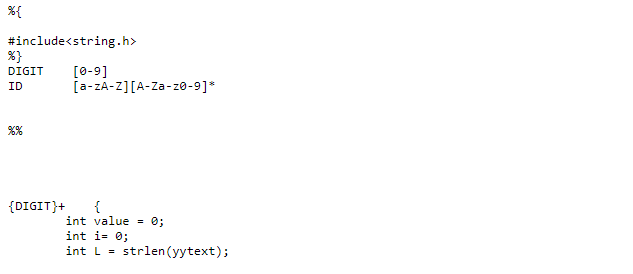
\includegraphics[scale=1]{d1}
	%\caption{Compiler phases}
\end{figure}

\begin{figure}
	\centering
	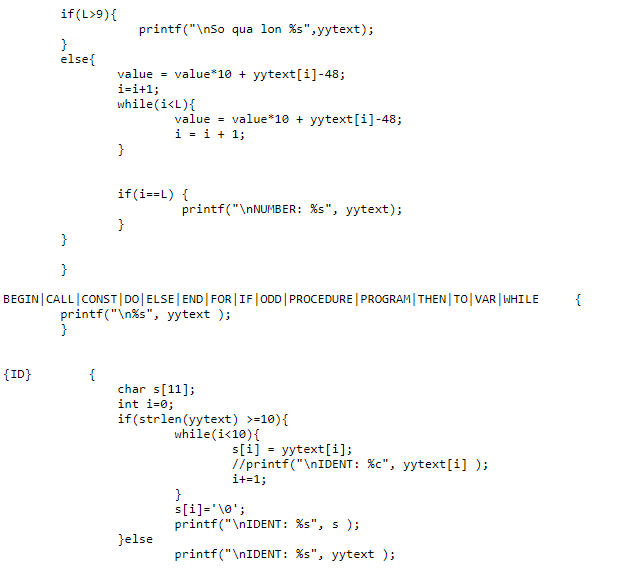
\includegraphics[scale=1]{d2}
	%\caption{Compiler phases}
\end{figure}

\begin{figure}
	\centering
	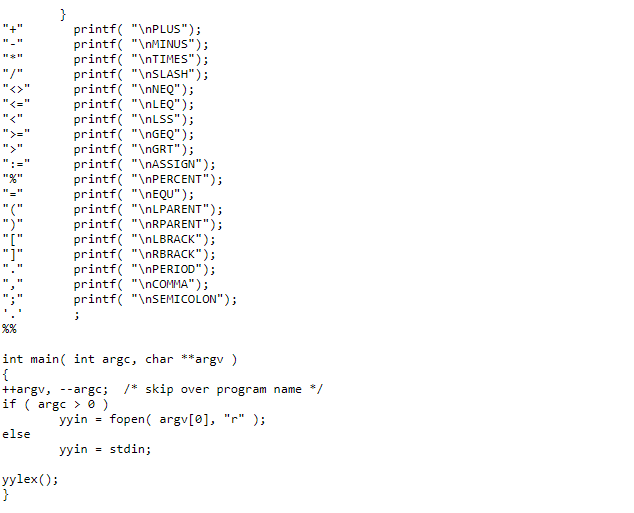
\includegraphics[scale=1]{d3}
	%\caption{Compiler phases}
\end{figure}

\newpage
Nếu ta chọn một file đầu vào để phân tích cú pháp như hình 5.1 thì ta sẽ thu được kết quả như hình 5.2 trên đây.

\begin{figure}
	\centering
	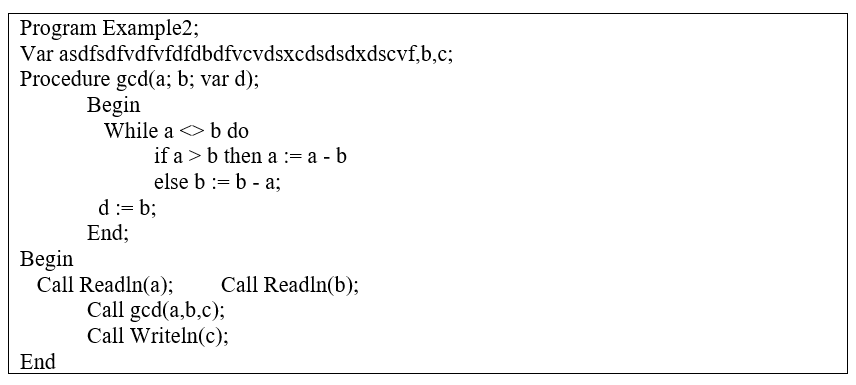
\includegraphics[scale=.6]{chuongtrinhcandich}
	\caption{Ví dụ file đầu vào}
\end{figure}


\begin{figure}
	\centering
	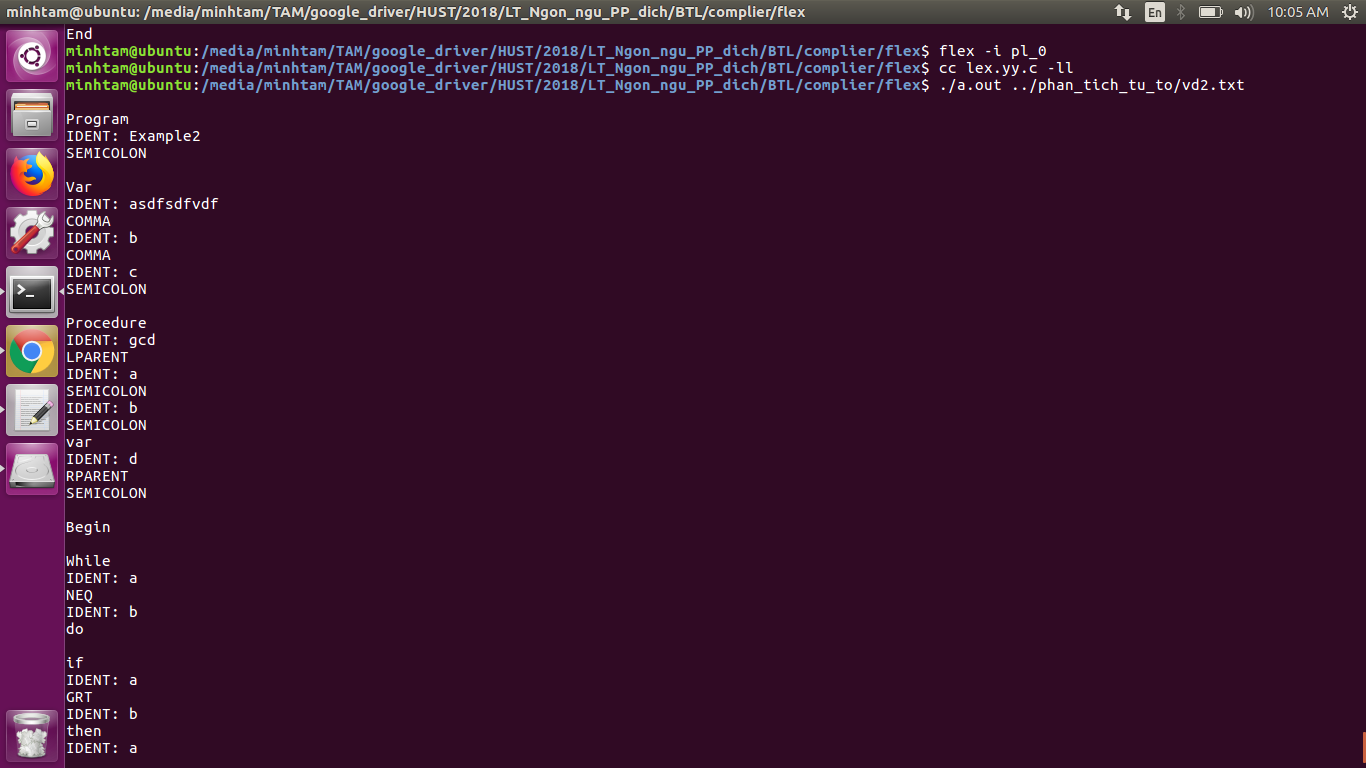
\includegraphics[scale=.39]{ketqua}
	\caption{Kết quả thu được khi chạy ví dụ}
\end{figure}

\begin{thebibliography}{9}
	\bibitem{latexcompanion} 
	Jonathan Engelsma.
	\textit{Part 01: Tutorial on lex/yacc}. 
	\textit{https://www.youtube.com/watch?v=54bo1qaHAfk\&t=746s}.
	
	
	\bibitem{latexcompanion} 
	\textit{Lexical Analysis With Flex, for Flex 2.6.2}.  
	\textit{http://westes.github.io/flex/manual/}.
	
	
	\bibitem{latexcompanion} 
	Phạm Đăng Hải.  
	\textit{Ngôn ngữ và phương pháp dịch}.  

	
	
	
\end{thebibliography}

\end{document}